% !TeX program = xelatex
% project_id: guardsynth-coc
% Main talk: 27 minutes; coauthor discussion: 3 minutes; backup slides untimed.
\documentclass[aspectratio=169,11pt]{beamer}
\usepackage{fontspec}
\setsansfont{TeX Gyre Heros}
\setmainfont{TeX Gyre Heros}
\setmonofont{Latin Modern Mono}
\usepackage{amsmath,amssymb,booktabs,array,tikz,pgfplots}
\newcolumntype{L}[1]{>{\raggedright\arraybackslash}p{#1}}
\usetikzlibrary{arrows.meta,positioning,calc}
\pgfplotsset{compat=1.18}
\definecolor{navy}{HTML}{142D4E}
\definecolor{teal}{HTML}{087E8B}
\definecolor{amber}{HTML}{B36D15}
\definecolor{muted}{HTML}{586776}
\definecolor{paperbg}{HTML}{F3F6F8}
\definecolor{danger}{HTML}{B34141}
\setbeamercolor{normal text}{fg=navy,bg=white}
\setbeamercolor{structure}{fg=teal}
\setbeamercolor{frametitle}{fg=navy}
\setbeamercolor{framesubtitle}{fg=muted}
\setbeamercolor{block title}{fg=navy,bg=teal!12}
\setbeamercolor{block body}{fg=navy,bg=paperbg}
\setbeamercolor{alerted text}{fg=danger}
\setbeamerfont{frametitle}{size=\Large,series=\bfseries}
\setbeamerfont{framesubtitle}{size=\small}
\setbeamerfont{block title}{size=\normalsize,series=\bfseries}
\setbeamertemplate{navigation symbols}{}
\setbeamertemplate{itemize item}{\color{teal}\small\raisebox{.2ex}{\(\blacktriangleright\)}}
\setbeamertemplate{itemize subitem}{\color{teal}\(\bullet\)}
\setbeamersize{text margin left=9mm,text margin right=9mm}
\setbeamertemplate{footline}{%
  \hspace{9mm}\begin{minipage}{.78\paperwidth}\color{muted}\scriptsize
  GuardSynth · \insertsectionhead
  \end{minipage}\hfill\color{muted}\scriptsize
  \ifnum\value{framenumber}<30 \insertframenumber/29\else Backup B\number\numexpr\value{framenumber}-29\relax\fi
  \hspace{8mm}\vspace{3mm}}
\ifdefined\seminarnotes
  \setbeameroption{show only notes}
\else
  \setbeameroption{hide notes}
\fi
\setbeamertemplate{note page}[plain]
\newcommand{\source}[1]{\par\vspace{2mm}{\fontsize{8}{10}\selectfont\color{muted}Source: #1\par}}
\newcommand{\takeaway}[1]{\begin{block}{Key message}#1\end{block}}
\newcommand{\good}[1]{\textcolor{teal}{#1}}
\newcommand{\bad}[1]{\textcolor{danger}{#1}}
\newcommand{\res}[2]{#1\,/\,\textcolor{muted}{#2}}
\tikzset{card/.style={rounded corners=2pt,draw=teal!35,fill=paperbg,align=center,inner sep=8pt},arr/.style={-{Stealth[length=2.3mm]},thick,teal}}
\title[GuardSynth]{GuardSynth: Augmenting Chain-of-Causation with Verified Behavioral Constraints for Autonomous Driving}
\subtitle{}
\author{Coauthor seminar}
\date{October 7, 2026}

\newcommand{\paperref}[2]{\href{#1}{\textcolor{teal}{#2}}}



\begin{document}

% TIMING 01 0.50

\begin{frame}[plain]
  \vspace{4mm}
  {\color{navy}\Huge\bfseries GuardSynth}\par\vspace{3mm}
  {\Large Augmenting Chain-of-Causation with\\Verified Behavioral Constraints\\for Autonomous Driving}\par\vfill
\note{\textbf{01 · Title · 0:00--0:30}\par Introduce the paper and its central idea: retain the action rationale, add an explicit restriction, and make the restriction traceable through specification, checking, and readable text. Follow the five sections shown by the section labels.}
\end{frame}

\section{1. Introduction}

% TIMING 02 1.00

\begin{frame}{Background: driving explanations need explicit conditions}
\begin{columns}[T,onlytextwidth]
\begin{column}{.57\textwidth}
\begin{block}{Context}
\begin{itemize}\setlength{\itemsep}{3mm}
\item VLMs: scene information → action choice
\item CoC: causal explanation for the action
\item Example: yield to a pedestrian, then proceed
\end{itemize}
\end{block}
\begin{block}{Missing detail}
When is proceeding \textbf{permitted}?
\end{block}
\end{column}
\begin{column}{.39\textwidth}
\begin{block}{Talk structure}
\begin{enumerate}\setlength{\itemsep}{3mm}
\item Introduction
\item Related work and comparison
\item Approach and verification
\item Experimental results
\item Conclusion
\end{enumerate}
\end{block}
\end{column}
\end{columns}
\source{Manuscript I; III; IV.A}
\note{\textbf{02 · Background: driving explanations need explicit conditions · 0:30--1:30}\par CoC means Chain of Causation and VLM means vision-language model. Our context is explaining and selecting driving actions. A rationale can explain why to yield without stating the clearance condition or waiting duration for later entry. Introduce the five-part outline before defining that gap.}
\end{frame}

% TIMING 03 0.75

\begin{frame}{Problem: turn an action rationale into a checkable restriction}
\begin{block}{Given}
CoC rationale + observations + supplied rules + modeling assumptions
\end{block}
\begin{block}{Required output}
\begin{itemize}\setlength{\itemsep}{2mm}
\item Explicit condition: \textbf{when} a restriction applies
\item Action restriction: \textbf{which} actions are prohibited
\item Release rule: \textbf{when} the restriction ends
\end{itemize}
\end{block}
\begin{itemize}\setlength{\itemsep}{2mm}
\item Avoid invented thresholds or unconfirmed scene facts.
\item Preserve allowed and forbidden behavior during conversion.
\end{itemize}
\source{Manuscript III; IV.A--B}
\note{\textbf{03 · Problem: turn an action rationale into a checkable restriction · 1:30--2:15}\par The task is constraint development, rather than choosing a trajectory directly. Inputs supply facts and normative rules. We seek a condition, action restriction, and release interpretation that can be checked before the restriction becomes a model-facing sentence. Neither an observed clearance time nor a rationale supplies a waiting duration by itself.}
\end{frame}

% TIMING 04 1.25

\begin{frame}{Approach and contributions}
  \framesubtitle{Each stage has a distinct output and responsibility}
  \vspace{1.5mm}
  \begin{center}
  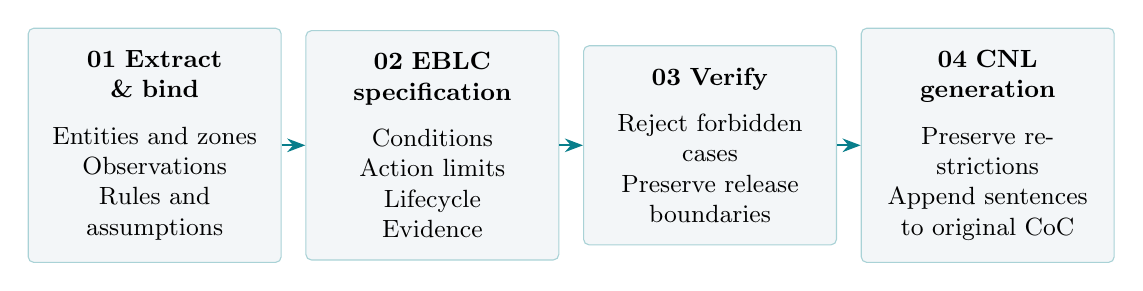
\begin{tikzpicture}[node distance=3mm]
    \node[card,font=\small,text width=2.65cm,minimum height=2.5cm] (a) {\textbf{01 Extract \& bind}\\[2mm]Entities and zones\\Observations\\Rules and assumptions};
    \node[card,font=\small,text width=2.65cm,minimum height=2.5cm,right=of a] (b) {\textbf{02 EBLC}\\\textbf{specification}\\[2mm]Conditions\\Action limits\\Lifecycle\\Evidence};
    \node[card,font=\small,text width=2.65cm,minimum height=2.5cm,right=of b] (c) {\textbf{03 Verify}\\[2mm]Reject forbidden\\cases\\Preserve release\\boundaries};
    \node[card,font=\small,text width=2.65cm,minimum height=2.5cm,right=of c] (d) {\textbf{04 CNL}\\\textbf{generation}\\[2mm]Preserve restrictions\\Append sentences\\to original CoC};
    \draw[arr] (a)--(b);\draw[arr] (b)--(c);\draw[arr] (c)--(d);
  \end{tikzpicture}
  \end{center}
  \begin{itemize}\small\setlength{\itemsep}{1mm}
    \item \textbf{Representation}: evidence-linked EBLC with defined lifecycle semantics
    \item \textbf{Assurance}: logical queries and source/representation checks
    \item \textbf{Learning interface}: readable CNL appended to the original CoC
  \end{itemize}
  \source{Manuscript Figure 1; IV.A--E}
\note{\textbf{04 · Approach and contributions · 2:15--3:30}\par Introduce EBLC as Evidence-Bound Lifecycle Contracts and CNL as Controlled Natural Language. Three contributions are the traceable representation, explicit checks, and a readable constraint interface for learning. The formal development path builds on our earlier natural-language guards; it is not a new universal traffic language. The experimental evidence concerns supplied synthetic rules.}
\end{frame}

\section{2. Related Work and Comparison}

% TIMING 05 1.00

\begin{frame}{Driving research: objectives and comparison}
  \framesubtitle{Compare central objectives; the studies use different benchmarks}
  \vspace{1.5mm}
  \renewcommand{\arraystretch}{1.18}\small
  \begin{tabular}{@{}L{3.5cm}L{4.7cm}L{4.7cm}@{}}
    \toprule
    \textbf{Study} & \textbf{Central approach} & \textbf{Relation to GuardSynth}\\\midrule
    \paperref{https://arxiv.org/abs/2312.14150}{DriveLM} & Graph VQA: perception, prediction, planning & Structure multi-step driving reasoning\\
    \paperref{https://arxiv.org/abs/2402.12289}{DriveVLM} & Scene analysis; hierarchical planning & Connect scene descriptions to plans\\
    \paperref{https://arxiv.org/abs/2511.00088}{Alpamayo-R1}; \paperref{https://ojs.aaai.org/index.php/AAAI/article/view/37602}{Drive-R1} & Reasoning/action alignment; SFT and RL & Link reasoning to action prediction\\
    \paperref{https://ojs.aaai.org/index.php/AAAI/article/view/41168}{DriveReg} & Retrieve regulations; reason with LLMs & Retrieve applicable rule evidence\\\bottomrule
  \end{tabular}\par
  \vspace{2mm}\normalsize
  \textbf{GuardSynth: specify → check → CNL}, developing the constraint component of learning inputs.
  \source{Manuscript II.A--B; Table 1. Study names link to primary sources.}
\note{\textbf{05 · Driving research: objectives and comparison · 3:30--4:30}\par Use the rows to locate our contribution, not to rank performance. SFT means supervised fine-tuning; RL means reinforcement learning; VQA means visual question answering. DriveLM structures reasoning through graph questions; DriveVLM organizes scene analysis and planning. Alpamayo-R1 and Drive-R1 emphasize reasoning/action alignment. DriveReg connects regulation retrieval with decisions. GuardSynth examines the constraint-development interface that can accompany a rationale. We have not run those systems on our candidate-selection benchmark and make no numerical superiority claim.}
\end{frame}

% TIMING 06 1.00

\begin{frame}{Formalization research: comparison and positioning}
  \framesubtitle{From formal rules and language translation to CoC learning inputs}
  \vspace{1.5mm}
  \renewcommand{\arraystretch}{1.16}\small
  \begin{tabular}{@{}L{3.2cm}L{4.5cm}L{5.2cm}@{}}
    \toprule
    \textbf{Study / approach} & \textbf{Central objective} & \textbf{GuardSynth's emphasis}\\\midrule
    \paperref{https://arxiv.org/abs/2007.00330}{Esterle et al.} & Traffic rules formalized in LTL & Evidence-linked constraints for CoC\\
    \paperref{https://aclanthology.org/2023.emnlp-main.985/}{NL2TL}\newline\paperref{https://arxiv.org/abs/2303.04864}{nl2spec} & Learned NL-to-logic translation; interactive correction & Supplied inputs mapped to restricted EBLC profiles\\
    \paperref{https://attempto.ifi.uzh.ch/site/pubs/papers/FLAIRS0601FuchsN.pdf}{ACE} & Controlled grammar with formal interpretation & Profile-specific CNL templates, distinct from ACE\\
    Our preceding CoC manuscript & Natural-language guards and contract-pair tasks & Source → fields → logic → CNL traceability\\\bottomrule
  \end{tabular}\par
  \vspace{2mm}\normalsize
  P1 is our earlier guard approach; P2 adds a \textbf{traceable EBLC development path}.
  \source{Manuscript II.C--E; Table 1. Table 2: native translation examples checked; no shared-task benchmark.}
\note{\textbf{06 · Formalization research: comparison and positioning · 4:30--5:30}\par LTL means Linear Temporal Logic; ACE means Attempto Controlled English. Traffic-rule formalization, learned translation, interactive correction, and controlled language are foundations rather than absent features in the field. Our contribution is their restricted, traceable connection to CoC learning inputs. The preceding manuscript already provides natural-language guards and the task families; do not claim those ideas are newly introduced here. P1 and P2 are internal development paths. Native checks ran one nl2spec CLI example with three translation samples and eleven official NL2TL notebook examples. They do not produce candidate-selection benchmark scores. DriveLM inference lacked the original LLaMA-7B weights locally; the inspected DriveVLM repository had no inference code or weights. Publication metadata for our preceding manuscript remains unconfirmed.}
\end{frame}

\section{3. Approach and Verification}

% TIMING 07 1.00

\begin{frame}{Constraint types: facts, reasons, restrictions, and goals}
  \framesubtitle{Only some CoC sentences express behavioral restrictions}
  \vspace{1.5mm}
  \renewcommand{\arraystretch}{1.12}\small
  \begin{tabular}{@{}L{2.25cm}L{7.7cm}L{3.1cm}@{}}
    \toprule
    \textbf{Role} & \textbf{Example} & \textbf{Purpose}\\\midrule
    Observation & A pedestrian occupies the conflict zone. & Describe a state\\
    Action rationale & Yield to protect the pedestrian. & Explain a reason\\
    Constraint & Do not enter while the zone is occupied. & Restrict allowed actions\\
    Objective & Choose the allowed action with the greatest progress. & Rank allowed actions\\\bottomrule
  \end{tabular}\par
  \vspace{3mm}\normalsize
  \takeaway{Meeting an entry condition permits entry; a separate objective chooses the action.}
  \source{Manuscript IV.B; IV.C, admissible candidate sets}
\note{\textbf{07 · Constraint types: facts, reasons, restrictions, and goals · 5:30--6:30}\par Read the example through four roles: what is present, why the vehicle yields, what actions are restricted, and which remaining action is preferred. A constraint does not replace an objective. This explains why a SAT candidate can still be an incorrect answer. We do not convert observations or objectives into invented rules.}
\end{frame}

% TIMING 08 1.00

\begin{frame}{Where do constraints come from?}
\vspace{1.5mm}
\renewcommand{\arraystretch}{1.1}\small
\begin{tabular}{@{}L{2.7cm}L{4.8cm}L{5.4cm}@{}}
\toprule
\textbf{Input} & \textbf{Synthetic experiment} & \textbf{Real-scene development}\\\midrule
Observation & Generated state/clearance & Video/annotation; human review\\
Rule & Supplied bounds or waiting duration & Rule evidence; applicability review\\
Assumption & Task: no reoccupation & Reviewed scene scope\\
Candidate values & Generated action summaries & Supported measurements needed\\\bottomrule
\end{tabular}\par
\vspace{1mm}\normalsize
\begin{block}{Six evaluated restrictions}
Speed cap · minimum clearance · minimum entry delay\\
Clearance + waiting · stopping bounds · lane-change gap
\end{block}
\small Human review: entities, zones, events, and rule applicability.\par
\source{Manuscript IV.B; Table 8; V.A}
\note{\textbf{08 · Where do constraints come from? · 6:30--7:30}\par Distinguish the source of every value. The synthetic experiment receives observations from the environment generator and thresholds from supplied rules. CoC identifies action-relevant content, but does not discover a traffic law or waiting duration from pixels. Real-scene development requires human confirmation of entities, zones, events, and rule applicability. Candidate measurements for that path are also needed and are not provided by the synthetic benchmark scores. The six task names describe restricted profiles, not complete real-road coverage.}
\end{frame}

% TIMING 09 1.00

\begin{frame}{EBLC: fields, lifecycle, and evidence}
  \framesubtitle{Evidence-Bound Lifecycle Contracts}
  \vspace{1.5mm}
  \renewcommand{\arraystretch}{1.2}\small
  \begin{tabular}{@{}L{2.8cm}L{10.2cm}@{}}
    \toprule
    \textbf{Element} & \textbf{Meaning in the pedestrian example}\\\midrule
    Target & The constrained vehicle and the pedestrian conflict zone\\
    Activation condition & A pedestrian occupies the zone.\\
    Action restriction & Prohibit the vehicle from entering the zone.\\
    Persistence & Retain the restriction until release is confirmed.\\
    Release & Confirm clearance and satisfy the supplied waiting duration.\\
    Evidence and scope & Occupancy/clearance evidence, rule source, no reoccupation, version\\\bottomrule
  \end{tabular}\par
  \vspace{2mm}\normalsize
  \textcolor{muted}{The paper implements \textbf{restricted profiles} with defined semantics. Coverage of every traffic situation has not been evaluated.}
  \source{Manuscript IV.C; Table 4; Code Box 1}
\note{\textbf{09 · EBLC: fields, lifecycle, and evidence · 7:30--8:30}\par Evidence-Bound means explicit links to the inputs on which a restriction depends. Lifecycle covers activation, persistence, release, and possible reactivation. A profile defines an interpretation beyond JSON fields. We do not claim a complete universal traffic-rule language. The primary temporal profile and qualitative lifecycle profile are separate implementations.}
\end{frame}

% TIMING 10 1.00

\begin{frame}{Temporal restriction: rules and candidate values}
  \framesubtitle{EBLC → Core logical representation → SMT; bind contract and candidate values}
  \vspace{1.5mm}
  \begin{block}{Restriction}
    \centering\Large\(e \Rightarrow u_{\mathrm{ms}}\geq\tau_{\mathrm{ms}}+\Delta_{\mathrm{ms}}\)
  \end{block}
  \renewcommand{\arraystretch}{1.25}\small
  \begin{tabular}{@{}llL{7.2cm}@{}}
    \(e\) & \texttt{enters} & Whether the candidate enters\\
    \(u_{\mathrm{ms}}\) & \texttt{entry\_ms} & The candidate's entry time\\
    \(\tau_{\mathrm{ms}}\) & \texttt{clear\_ms} & Environmental clearance time\\
    \(\Delta_{\mathrm{ms}}\) & \texttt{release\_clear\_ms} & Minimum waiting duration specified in EBLC\\
  \end{tabular}\par
  \normalsize
  \takeaway{A candidate with \(e=\mathrm{false}\) satisfies this entry restriction. Its progress is scored separately.}
  \source{Manuscript IV.C, temporal semantics; IV.D, Core lowering}
\note{\textbf{10 · Temporal restriction: rules and candidate values · 8:30--9:30}\par Define all four symbols. Entry and entry time belong to the candidate; clearance belongs to the environment; waiting duration belongs to the contract. Core is a typed intermediate representation compiled to SMT. The check uses integer milliseconds, not a continuous vehicle trajectory. With enters=false the implication holds, but this does not make the candidate preferable.}
\end{frame}

% TIMING 11 1.00

\begin{frame}{Verification method: specification → logic → queries}
\begin{enumerate}\setlength{\itemsep}{3mm}
\item \textbf{Bind inputs}\par
\small Same entity, zone, event, rule, and case; confirm units/version.\normalsize
\item \textbf{Compile EBLC → Core → SMT}\par
\small Core: typed declarations and logical clauses.\normalsize
\item \textbf{Run allowed / forbidden queries}\par
\small Compare expected SAT/UNSAT with solver results.\normalsize
\item \textbf{Check correspondence}\par
\small Source $\leftrightarrow$ EBLC $\leftrightarrow$ rule calculation $\leftrightarrow$ CNL.\normalsize
\end{enumerate}
\begin{block}{Review trigger}
Unexpected SAT/UNSAT or solver UNKNOWN → review and recheck
\end{block}
\source{Manuscript IV.D--E; Table 6; VI.G}
\note{\textbf{11 · Verification method: specification → logic → queries · 9:30--10:30}\par SMT means Satisfiability Modulo Theories. This slide concerns the specification and conversion pipeline before learning. Validate field combinations and semantic bindings, compile the restricted contract, and probe both allowed and forbidden behavior. SAT is an existing satisfying assignment; UNSAT excludes the queried assignment. Multiple checks contribute to correspondence; factual truth of video or adequacy of a supplied threshold is not proved by SAT. Model prediction evaluation appears later.}
\end{frame}

% TIMING 12 1.00

\begin{frame}{Verification properties and executed temporal results}
  \framesubtitle{Temporal example: clearance 11.0 s; required wait 0.5 s}
  \vspace{1.5mm}
  \renewcommand{\arraystretch}{1.05}\small
  \begin{tabular}{@{}L{2.5cm}L{6.5cm}L{3.9cm}@{}}
    \toprule
    \textbf{Property} & \textbf{Query} & \textbf{Expected result}\\\midrule
    Consistency & Does a satisfying assignment exist? & SAT\\
    Enforcement & Any entering assignment before release? & UNSAT\\
    Release boundary & Entry at 11.499 / 11.500 / 11.501 s & UNSAT / SAT / SAT\\
    Deferral & A candidate that defers entry & SAT\\\bottomrule
  \end{tabular}\par
  \vspace{1mm}\normalsize
  \begin{block}{Executed results}
Six queries × two waiting contracts = \good{12 matching verdicts}.\\
Separate archive: 100 bridge queries rerun.
\end{block}
\small Safety: exclude premature entry. Feasibility: permit released entry.\\
\textbf{Liveness is not established}: deferral remains allowed.
  \source{Manuscript Table 6; IV.D, Properties and Queries}
\note{\textbf{12 · Verification properties and executed temporal results · 10:30--11:30}\par Use the table to define consistency, restriction enforcement, release boundaries, and deferral. The manuscript ran all six queries for both 500 ms and 1500 ms waiting contracts, giving twelve matching verdicts. The existing bridge has a separate set of one hundred rerun queries; do not pool it as new learning evidence. Early-entry UNSAT excludes a hypothetical forbidden assignment, not an observed violation. SAT at release establishes feasibility, not eventual progress or liveness.}
\end{frame}

% TIMING 13 1.00

\begin{frame}{Lifecycle verification: persistence, release, and reactivation}
  \framesubtitle{A separate profile from the primary temporal learning experiment}
  \vspace{1.5mm}
  \begin{block}{Current evidence and previous activation}
    \centering
    \(\mathrm{active}_{j,t}=\begin{cases}
      \mathrm{true} & \text{valid TRUE}\\
      \mathrm{false} & \text{valid FALSE}\\
      \mathrm{active}_{j,t-1} & \text{UNKNOWN, CONFLICT, invalid evidence}
    \end{cases}\)
  \end{block}
  \begin{center}
    \begin{tabular}{@{}lcccc@{}}
      Evidence & TRUE & UNKNOWN & FALSE & TRUE\\
      Activation & Active & Retained & Released & Reactivated\\
    \end{tabular}\par
  \end{center}
  \begin{itemize}\small\setlength{\itemsep}{1mm}
\item Constructed-history checks: persistence, invalid-evidence retention, release, reactivation.
\item Active + UNKNOWN + forced inactive → \good{UNSAT}.
\item Initial state supplied; entry requires current valid clearance for every obligation.
\end{itemize}
  \source{Manuscript Code Box 2; Figure 3; IV.D, Lifecycle Checks}
\note{\textbf{13 · Lifecycle verification: persistence, release, and reactivation · 11:30--12:30}\par This is a separate qualitative profile. Truth records the evidence status; active records whether the obligation applies. Valid TRUE activates, valid FALSE releases, and UNKNOWN, CONFLICT, or invalid evidence retains prior activation. The executed checks use constructed sequences and supplied initial states. Forcing an active obligation inactive under UNKNOWN is UNSAT. These checks validate the encoded transition interpretation, not automatic recovery of real road history.}
\end{frame}

% TIMING 14 1.00

\begin{frame}{Verification results: which layer detects each error?}
\framesubtitle{192 balanced cases; specification quality is separate from model selection}
\renewcommand{\arraystretch}{1.13}\small
\begin{tabular}{@{}L{5.8cm}L{2.2cm}L{4.7cm}@{}}
\toprule
\textbf{Mutation / input} & \textbf{Detected / cases} & \textbf{Checking layer}\\\midrule
CNL negation / CNL threshold & 24/24 each & CNL correspondence\\
Release deletion / reversed comparison & 24/24 each & Core--environment\\
Specification threshold change & 24/24 & Source + Core\\
Incorrect unit & 24/24 & Schema\\
Shared source/specification error & \bad{0/24} & No layer detects it\\
Valid contract & --- & 24/24 accepted\\
\bottomrule\end{tabular}\par
\normalsize
\vspace{2mm}
\begin{itemize}\small\setlength{\itemsep}{1.5mm}
\item Balanced set: 192 cases; 144 of 168 errors detected (85.71\%).
\item Checks accept 48 cases: 24 valid + 24 shared-source errors.
\item A wrong wait copied consistently from the source can remain SAT.
\end{itemize}
\source{Manuscript Table 15; V.A.5; VI.G; Supplement S3}
\note{\textbf{14 · Verification results: which layer detects each error? · 12:30--13:30}\par Six supported mutation categories each have twenty-four cases. All one hundred forty-four are detected, but the layer matters. CNL changes need sentence-to-specification correspondence, units need schema checking, and release or comparison changes need the Core and reference-rule comparison. Twenty-four shared-source errors remain undetected because source and specification change together; all remain internally SAT. Twenty-four valid contracts are accepted without false rejection. Bypassing checks accepts all one hundred ninety-two cases, while checking retains forty-eight. This is a balanced injected-error study, not a natural error rate or a SAT-only success rate. The records are reused once, without claiming a new experiment.}
\end{frame}

% TIMING 15 1.00

\begin{frame}{Output: original CoC + verified constraint sentences}
  \framesubtitle{Controlled Natural Language: original CoC followed by generated restrictions}
  \vspace{1.5mm}
  \begin{block}{Original CoC}
    \small Yield to the crossing pedestrian, then proceed through the intersection.
  \end{block}
  \begin{block}{CNL generated from EBLC}
    \small Do not enter the pedestrian conflict zone while it is occupied.\\[2mm]
    Enter only after the zone has remained clear for at least 0.5 s.
  \end{block}
  \begin{itemize}\small\setlength{\itemsep}{1mm}
    \item “At least” preserves \(\geq\); “only after” states a necessary condition for entry.
    \item Separate records: EBLC, evidence, solver verdicts, and reference labels.
  \end{itemize}
  \source{Manuscript Table 7; Figure 4; IV.E}
\note{\textbf{15 · Output: original CoC + verified constraint sentences · 13:30--14:30}\par Read the original rationale followed by the generated restrictions. At least preserves the inclusive boundary; only after states a necessary condition, not a command to enter. This text is inserted into Requirement CoC before candidate descriptions. The image, environmental information, and action candidates accompany it. The model predicts A through D; the reference label is a supervised target, not a prompt hint. Raw EBLC and solver verdicts remain in separate records.}
\end{frame}

\section{4. Experimental Results}

% TIMING 16 1.00

\begin{frame}{Experimental comparison: P0, P1, and P2}
  \framesubtitle{Primary comparison: constraint-conditioned P1/P2 versus CoC-only P0}
  \vspace{1.5mm}
  \renewcommand{\arraystretch}{1.10}\small
  \begin{tabular}{@{}lL{5.9cm}L{5.5cm}@{}}
    \toprule
    Condition & Model-facing content & Role\\\midrule
    P0 & Original CoC & Baseline without the constraint\\
    P1 & CoC + existing natural-language constraint & Existing natural-language path\\
    P2 & CoC + EBLC-derived CNL & Specification and verification path\\\bottomrule
  \end{tabular}\par
  \vspace{3mm}\normalsize
  \begin{itemize}\setlength{\itemsep}{2mm}
    \item Images, candidates, labels, and splits are shared. P1/P2 receive constraints at training and evaluation.
    \item P0 cannot distinguish 0.5 s from 1.5 s rules for an otherwise identical input.
  \end{itemize}
  \takeaway{This tests \textbf{supplied-constraint use}, not a separate causal benefit of verification.}
  \source{Manuscript Table 9; V.A; VII.A--B}
\note{\textbf{16 · Experimental comparison: P0, P1, and P2 · 14:30--15:30}\par P1/P2 are our development paths, not external competitors. Gains over P0 include additional rule information. Constraints appear during training and evaluation, so this is not testing compliance without evaluation-time constraints. P2 is not consistently more accurate than P1. Agreeing on this scope is important for the paper's positioning.}
\end{frame}

% TIMING 17 0.50

\begin{frame}{Comparison scope: external systems and prompting controls}
\framesubtitle{Direct performance comparisons with the four external systems were not conducted}
\begin{block}{Why direct comparison was not performed}
\begin{itemize}\small\setlength{\itemsep}{1mm}
\item nl2spec / NL2TL: logic-translation outputs differ from our A--D selection task.
\item DriveLM / DriveVLM: required weights or inference code were unavailable in the inspected setup.
\end{itemize}
\end{block}
\begin{block}{What we measured on our task}
\begin{itemize}\small\setlength{\itemsep}{1mm}
\item \textbf{P0 + ZS-CoT:} Zero-Shot Chain-of-Thought; request step-by-step reasoning.
\item \textbf{P0 + PS:} basic Plan-and-Solve; request a plan, then solve step by step.
\end{itemize}
\small Same P0 checkpoints and inputs; added inference instructions only.\\[1mm]
480 rows × 3 seeds × 2 methods = 2,880 predictions; no added rules or training.
\end{block}
\small Adapted prompting, not original-benchmark reproduction. Results: slide 20.
\source{Manuscript V.A.4; VI.B; Table 2; execution checks in backup B9}
\note{\textbf{17 · Comparison scope: external systems and prompting controls · 15:30--16:00}\par We did not measure our candidate-selection accuracy against nl2spec, NL2TL, DriveLM, or DriveVLM. Original example executions are availability checks only and remain in B9. P0 plus ZS-CoT means the existing CoC-only P0 checkpoint with a Zero-Shot Chain-of-Thought instruction at inference. P0 plus PS uses that same checkpoint with the basic Plan-and-Solve instruction to devise a plan and carry it out step by step. The plus sign denotes added prompting, not a newly trained model, extra constraints, or an ensemble. Results appear on slide twenty. These controls transfer prompting procedures to our task; they do not reproduce the original benchmarks.}
\end{frame}

% TIMING 18 1.00

\begin{frame}{Evaluation design: datasets, model, and metrics}
  \framesubtitle{Rows per P0/P1/P2 condition; three optimization seeds}
  \vspace{1.5mm}
  \renewcommand{\arraystretch}{1.35}\small
  \begin{tabular}{@{}lrrrL{4.6cm}@{}}
    \toprule
    Family & Training & Validation & Primary test & Tasks\\\midrule
    Temporal & 960 & 240 & 240 & Entry after clearance and waiting\\
    Static & 576 & --- & 144 & Speed, clearance, entry delay\\
    Maneuver & 384 & --- & 96 & Stopping and lane change\\\bottomrule
  \end{tabular}\par
  \vspace{4mm}\normalsize
  \begin{itemize}\setlength{\itemsep}{2mm}
    \item Qwen3-VL-2B-Instruct + LoRA; 3 epochs; seeds 42, 17, 123.
    \item Accuracy: highest-progress allowed answer; violation: prohibited choice.
    \item Pair accuracy: both rule variants correct. Numeric candidates supplied in text.
  \end{itemize}
  \source{Manuscript Table 10; V.A.1--3; Supplement S1, S8}
\note{\textbf{18 · Evaluation design: datasets, model, and metrics · 16:00--17:00}\par Each example gives an image, CoC text, and four candidate descriptions. A separate program applies the supplied rule and selects the allowed candidate with greatest synthetic utility as the reference label. The model is trained to output A, B, C, or D. Accuracy measures this label match; violation checks whether the predicted candidate is forbidden; pair accuracy requires both rule variants correct. The primary test has 480 rows per condition, not 480 independent videos. Each static subtype, stopping, and lane change has 48 test rows. Static and maneuver families use final checkpoints without validation sets.}
\end{frame}

% TIMING 19 1.50

\begin{frame}{Primary results: accuracy and constraint violations}
  \framesubtitle{Six tasks · P0/P1/P2 · means over three seeds}
  \vspace{1.5mm}
\begin{columns}[T,onlytextwidth]
\begin{column}{.49\textwidth}
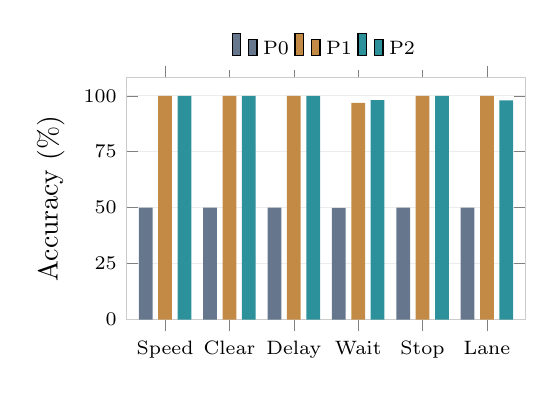
\begin{tikzpicture}
\begin{axis}[width=6.65cm,height=4.65cm,ybar,bar width=5pt,ymin=0,ymax=108,
symbolic x coords={Speed,Clear,Delay,Wait,Stop,Lane},xtick=data,ytick={0,25,50,75,100},
ylabel={Accuracy (\%)},tick label style={font=\scriptsize},
legend style={at={(.5,1.03)},anchor=south,legend columns=3,draw=none,font=\scriptsize},
ymajorgrids=true,grid style={gray!15},axis line style={gray!40},enlarge x limits=.12]
\addplot[fill=navy!65,draw=none] coordinates {(Speed,50) (Clear,50) (Delay,50) (Wait,49.86) (Stop,50) (Lane,50)};
\addplot[fill=amber!80,draw=none] coordinates {(Speed,100) (Clear,100) (Delay,100) (Wait,96.81) (Stop,100) (Lane,100)};
\addplot[fill=teal!85,draw=none] coordinates {(Speed,100) (Clear,100) (Delay,100) (Wait,98.06) (Stop,100) (Lane,97.92)};
\legend{P0,P1,P2}
\end{axis}\end{tikzpicture}
\end{column}
\begin{column}{.49\textwidth}
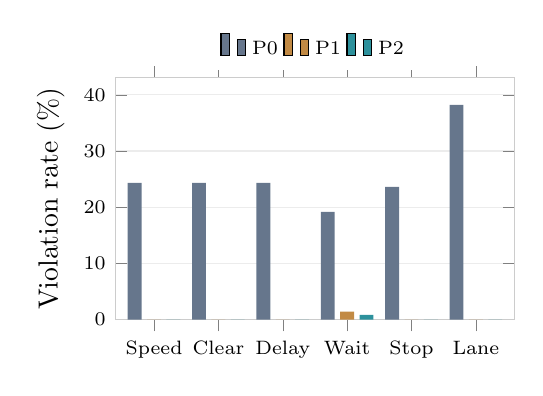
\begin{tikzpicture}
\begin{axis}[width=6.65cm,height=4.65cm,ybar,bar width=5pt,ymin=0,ymax=43,
symbolic x coords={Speed,Clear,Delay,Wait,Stop,Lane},xtick=data,ytick={0,10,20,30,40},
ylabel={Violation rate (\%)},tick label style={font=\scriptsize},
legend style={at={(.5,1.03)},anchor=south,legend columns=3,draw=none,font=\scriptsize},
ymajorgrids=true,grid style={gray!15},axis line style={gray!40},enlarge x limits=.12]
\addplot[fill=navy!65,draw=none] coordinates {(Speed,24.31) (Clear,24.31) (Delay,24.31) (Wait,19.17) (Stop,23.61) (Lane,38.19)};
\addplot[fill=amber!80,draw=none] coordinates {(Speed,0) (Clear,0) (Delay,0) (Wait,1.39) (Stop,0) (Lane,0)};
\addplot[fill=teal!85,draw=none] coordinates {(Speed,0) (Clear,0) (Delay,0) (Wait,0.83) (Stop,0) (Lane,0)};
\legend{P0,P1,P2}
\end{axis}\end{tikzpicture}
\end{column}
\end{columns}
\begin{itemize}\small\setlength{\itemsep}{1mm}
\item Wait task, P2: \textbf{98.06\% accuracy; 0.83\% violations}.
\item P1/P2 improve over P0; P2 does not consistently outperform P1.
\end{itemize}
\source{Manuscript Table 11; three-seed means; exact values in backup B6}
\note{\textbf{19 · Primary results: accuracy and constraint violations · 17:00--18:30}\par These two plots reproduce all six task rows from Table 11. Speed is maximum speed, Clear is minimum obstacle clearance, Delay is minimum entry delay, Wait is entry after clearance and waiting, Stop is stopping, and Lane is lane change. P1 and P2 outperform P0 in every task. P1 and P2 tie in the three static types and stopping. P2 temporal accuracy is 98.06 percent with 0.83 percent violations. Lane-change P2 is 97.92 percent versus P1 at 100 percent, and those residual P2 errors are allowed but lower-progress selections. The plots show means, not uncertainty intervals. Exact values remain in B6.}
\end{frame}

% TIMING 20 1.00

\begin{frame}{Reasoning prompts without the missing rule}
\framesubtitle{Same P0 checkpoints and candidates; no additional training or constraint input}
\begin{center}\includegraphics[width=.92\textwidth,height=3.8cm,keepaspectratio]{projects/04-guardsynth-coc/paper/ieee-access/figures/reasoning-comparison-en.pdf}\end{center}
\vspace{-1mm}
\small \textbf{P0 + ZS-CoT:} Zero-Shot Chain-of-Thought; “Let's think step by step.”\\[1mm]
\textbf{P0 + PS:} basic Plan-and-Solve; plan first, then solve step by step.
\begin{itemize}\small\setlength{\itemsep}{1mm}
\item P0 / Zero-shot CoT / basic PS: pooled accuracy \textbf{49.93\%} each.
\item Violation rates: 23.06\% / 22.64\% / 22.71\%; pair accuracy 0\%.
\end{itemize}
\source{Manuscript Figure 5; V.A.4; VI.B; original prompting procedures transferred}
\note{\textbf{20 · Reasoning prompts without the missing rule · 18:30--19:30}\par The chart reproduces manuscript Figure 5 using archived results for all six tasks. P0 is the original CoC-only checkpoint. P0 plus ZS-CoT adds the instruction ``Let's think step by step.'' and uses a second generation to extract the answer. P0 plus PS adds the basic instruction to understand the problem, devise a plan, and carry it out step by step; answer extraction uses its answer tail or a further generation if the tail is absent. These are inference-time prompts on existing P0 checkpoints, without added rules or retraining. The reasoning token caps are one hundred twenty-eight for ZS-CoT and two hundred fifty-six for PS, so inference budgets are unequal. Each method evaluates two hundred forty temporal, one hundred forty-four static, and ninety-six maneuver rows for three seeds. Basic PS is not PS plus, and neither procedure uses self-consistency. Accuracy remains forty-nine point nine three percent, while violations change slightly. All unique ZS-CoT first stages emit option-label strings; PS does so in four hundred ninety-eight of five hundred forty-six unique cases, with forty-eight static cases reaching the reasoning cap. A reasoning instruction does not establish that these label-trained models actually carry out multistep reasoning. P1/P2 have additional rule information.}
\end{frame}

% TIMING 21 1.00

\begin{frame}{Contract-pair results: does the choice follow the changed rule?}
  \framesubtitle{Contract-pair accuracy requires both members of a pair to be correct}
  \vspace{1.5mm}
  \begin{columns}[T,onlytextwidth]
    \begin{column}{.69\textwidth}
      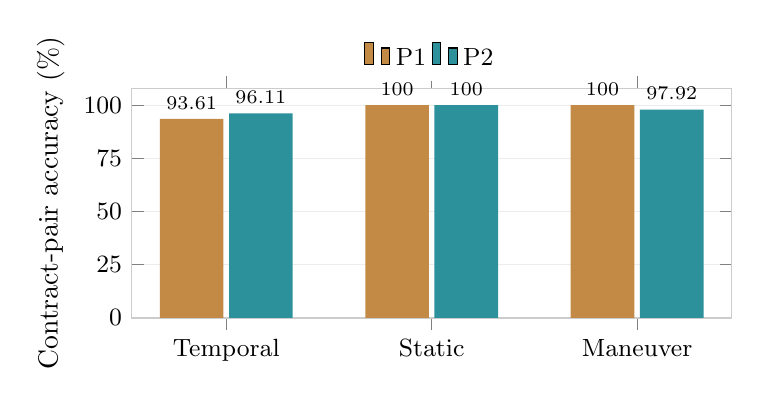
\begin{tikzpicture}
      \begin{axis}[width=9.2cm,height=4.5cm,ybar,bar width=23pt,ymin=0,ymax=108,
        symbolic x coords={Temporal,Static,Maneuver},xtick=data,ytick={0,25,50,75,100},
        ylabel={Contract-pair accuracy (\%)},tick label style={font=\small},
        legend style={at={(.5,1.03)},anchor=south,legend columns=2,draw=none,font=\small},
        ymajorgrids=true,grid style={gray!15},axis line style={gray!40},
        nodes near coords,every node near coord/.append style={font=\scriptsize},enlarge x limits=.23]
        \addplot[fill=amber!80,draw=none] coordinates {(Temporal,93.61) (Static,100) (Maneuver,100)};
        \addplot[fill=teal!85,draw=none] coordinates {(Temporal,96.11) (Static,100) (Maneuver,97.92)};
        \legend{P1,P2}
      \end{axis}
      \end{tikzpicture}
    \end{column}
    \begin{column}{.28\textwidth}\begin{block}{P0 = 0\%}
      All three families\\[2mm]
      P0 lacks the rule that distinguishes identical inputs with different answers.
    \end{block}\end{column}
  \end{columns}
  \source{Manuscript Figure 6, left; VI.C; Supplement S2, S8}
\note{\textbf{21 · Contract-pair results: does the choice follow the changed rule? · 19:30--20:30}\par Answering both variants is stronger than answering one case. Recall B under 0.5 seconds and C under 1.5 seconds. Zero P0 pair accuracy is not a general failure of CoC reasoning: identical P0 inputs have different labels. P1/P2 receive the distinguishing rule and usually change their choices correctly. These observations concern supplied-rule use, not new-scene visual generalization.}
\end{frame}

% TIMING 22 1.00

\begin{frame}{Association test: correct versus shuffled constraints}
\begin{columns}[T,onlytextwidth]
\begin{column}{.68\textwidth}
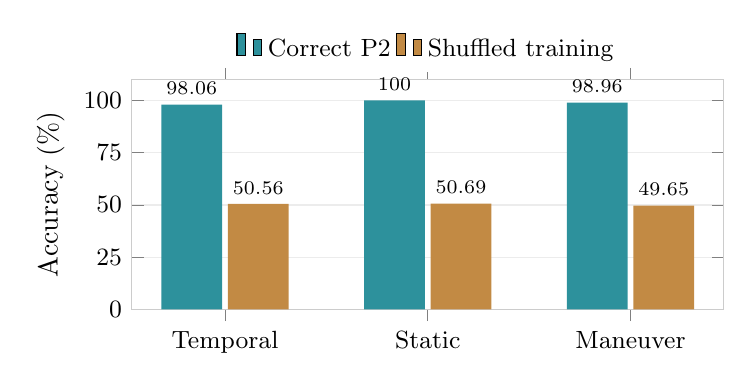
\begin{tikzpicture}
\begin{axis}[width=9.1cm,height=4.5cm,ybar,bar width=22pt,ymin=0,ymax=110,
symbolic x coords={Temporal,Static,Maneuver},xtick=data,ytick={0,25,50,75,100},
ylabel={Accuracy (\%)},tick label style={font=\small},
legend style={at={(.5,1.03)},anchor=south,legend columns=2,draw=none,font=\small},
ymajorgrids=true,grid style={gray!15},axis line style={gray!40},
nodes near coords,every node near coord/.append style={font=\scriptsize},enlarge x limits=.23]
\addplot[fill=teal!85,draw=none] coordinates {(Temporal,98.06) (Static,100) (Maneuver,98.96)};
\addplot[fill=amber!80,draw=none] coordinates {(Temporal,50.56) (Static,50.69) (Maneuver,49.65)};
\legend{Correct P2,Shuffled training}
\end{axis}\end{tikzpicture}
\end{column}
\begin{column}{.29\textwidth}
\begin{block}{Intervention}
\small Shuffle case--constraint links at training.\\[2mm]
Restore correct links at evaluation.
\end{block}
\textbf{Result}: accuracy near 50\% after shuffling.
\end{column}
\end{columns}
\source{Manuscript Figure 6, right; temporal intervention uses NL guards; others use P2 CNL}
\note{\textbf{22 · Association test: correct versus shuffled constraints · 20:30--21:30}\par The normal P2 performance is a reference for the shuffled-association intervention. Training associates the wrong constraint with each case; evaluation restores the correct constraint. Temporal shuffling uses natural-language guards, while static and maneuver shuffling uses P2 CNL within subtype. Thus the intervention is not identical across families. The fall toward fifty percent supports the importance of correct case--constraint associations, without isolating the contribution of SMT verification.}
\end{frame}

% TIMING 23 1.00

\begin{frame}{Constraint representation: accuracy and generalization}
\framesubtitle{Cells = accuracy / violation rate (\%); three-seed means}

\begin{columns}[T,onlytextwidth]
\begin{column}{.64\textwidth}
\renewcommand{\arraystretch}{1.13}\small
\begin{tabular}{@{}L{3.0cm}L{2.5cm}L{2.5cm}@{}}
\toprule
\textbf{Representation} & \textbf{Primary} & \textbf{Unseen wait}\\\midrule
P0 & \res{49.86}{19.17} & \res{49.86}{18.47}\\
P1 & \res{96.81}{1.39} & \res{96.67}{2.22}\\
P2 & \res{98.06}{0.83} & \res{96.67}{1.53}\\
Alternative NL & \res{98.06}{1.11} & \res{98.61}{0.56}\\
Shuffled NL & \res{50.56}{19.72} & \res{50.97}{18.89}\\
Logical text & \res{99.17}{0.14} & \res{81.25}{0.83}\\
\bottomrule\end{tabular}\par
\normalsize
\end{column}
\begin{column}{.32\textwidth}
\begin{block}{Matched temporal fits}\small
6 arms × 3 seeds\\
960 training rows\\
180 updates per fit\\
240 rows per test
\end{block}
\small Shuffled at training; correctly associated guards at evaluation.
\end{column}\end{columns}
\vspace{2mm}\small
\textbf{Logical text:} accuracy 99.17\% → 81.25\% on unseen waits.\\[1mm]
\textbf{Interpretation:} CNL does not dominate every alternative.

\source{Manuscript Table 12; V.A.5; VI.D; Supplement additional temporal analyses}
\note{\textbf{23 · Constraint representation: accuracy and generalization · 21:30--22:30}\par All six arms use the same temporal generator, training budget, and seeds. Alternative NL is the NATURAL\_GUARD arm; Shuffled NL is SHUFFLED\_GUARD; Logical text is LOGIC\_GUARD. They are model-input representations, not external systems. Unseen waits are zero point eight and one point eight seconds, versus zero point five and one point five during training. Logical text reaches the highest primary accuracy but drops substantially on new durations despite a low violation rate, because an allowed choice can still be suboptimal. Natural-language guards match or exceed P2 on some conditions. The contribution of EBLC is the traceable, checkable path, not universal behavioral superiority.}
\end{frame}

% TIMING 24 1.00

\begin{frame}{Wording changes and combined hard conditions}
\framesubtitle{Accuracy / violation rate (\%); original checkpoints, three seeds, no new training}
\renewcommand{\arraystretch}{1.13}\small
\begin{tabular}{@{}L{5.2cm}L{2.5cm}L{2.5cm}L{2.5cm}@{}}
\toprule
\textbf{Evaluation (rows)} & \textbf{P0} & \textbf{P1} & \textbf{P2}\\\midrule
Temporal paraphrase (240) & \res{49.86}{19.17} & \res{90.56}{5.00} & \res{96.94}{1.25}\\
Static paraphrase (144) & \res{50.00}{24.31} & \res{93.29}{0.00} & \res{80.32}{7.87}\\
Maneuver paraphrase (96) & \res{50.00}{30.90} & \res{100.00}{0.00} & \res{97.92}{2.08}\\
Combined hard maneuver (96) & \res{50.00}{30.21} & \res{94.10}{0.69} & \res{91.32}{1.04}\\
\bottomrule\end{tabular}\par
\normalsize
\vspace{2mm}
\begin{itemize}\small\setlength{\itemsep}{2mm}
\item Paraphrase: same cases and rules, changed constraint wording.
\item Static P2: primary 100\% / 0\% → paraphrase \bad{80.32\% / 7.87\%}.
\item Hard test combines negation, clause order, equality, and m/cm units.
\item New numerical values are a separate test (backup B7).
\end{itemize}
\source{Manuscript Table 13; V.A.5; VI.E; Supplement S5, S8--S9}
\note{\textbf{24 · Wording changes and combined hard conditions · 22:30--23:30}\par These rows are three-seed means, and the counts refer to rows per arm and seed, not independent videos. Temporal P1 and P2 receive the same held-out paraphrase; P0 receives unchanged inputs in the paraphrase conditions. P2 performs better than P1 on the temporal paraphrase, but worse on the static one. Static P2 drops from perfect primary performance to eighty point three two percent accuracy with seven point eight seven percent violations. The hard maneuver test combines four changes and cannot isolate individual causes; P2 has ninety-one point three two percent accuracy and one point zero four percent violations. Both favorable and unfavorable results are retained. The separate small follow-up wording diagnostic in S9 also shows failures: its second paraphrase gives P1/P2 accuracy seventy-six point three nine/seventy-seven point seven eight percent.}
\end{frame}

% TIMING 25 1.00

\begin{frame}{Visual-input diagnostic: remove or alter the image}
\framesubtitle{Cells = source-reference accuracy / violation rate (\%); three-seed means}
\renewcommand{\arraystretch}{1.13}\small
\begin{tabular}{@{}L{5.2cm}L{2.5cm}L{2.5cm}L{2.5cm}@{}}
\toprule
\textbf{Image condition} & \textbf{P0} & \textbf{P1} & \textbf{P2}\\\midrule
Original & \res{50.00}{22.22} & \res{100.00}{0.00} & \res{98.61}{1.39}\\
Blank & \res{50.00}{13.89} & \res{81.94}{2.78} & \res{76.39}{1.39}\\
Redrawn: clearance +1 s & \res{50.00}{19.44} & \res{87.50}{0.00} & \res{79.17}{1.39}\\
\bottomrule\end{tabular}\par
\normalsize
\vspace{2mm}
\begin{block}{Paired intervention}\small
24 rows: 3 semantic groups × 2 rules × 4 label rotations.\\
Keep text, candidates and source-reference labels fixed; change only the image.
\end{block}
\small
\textbf{P2 selection changes:} 25.00\% blank; 19.44\% redrawn.\\[1mm]
\textbf{Scope:} visual sensitivity; the conflicting-image scores are diagnostic.

\source{Manuscript Table 14; V.A.5; VI.F; Supplement S9}
\note{\textbf{25 · Visual-input diagnostic: remove or alter the image · 23:30--24:30}\par Nine existing P0/P1/P2 adapters run twenty-four rows in each of the original, blank, and redrawn conditions, yielding six hundred forty-eight predictions. These form part of the archived two thousand one hundred sixty follow-up predictions; there is no new training. Blank images remove scene information. Redrawn images show clearance one second later while the textual case and source-reference target are retained, creating an explicit input conflict. P2 source-reference accuracy decreases from ninety-eight point six one to seventy-six point three nine and seventy-nine point one seven percent. Its violation rate stays at one point three nine percent, so changed choices can be allowed but lower-progress. A response to visual change is not proof of correct event interpretation, and three semantic groups do not establish road perception accuracy.}
\end{frame}

% TIMING 26 1.00

\begin{frame}{Experimental interpretation: scope and limitations}
  \framesubtitle{Representation, wording, image dependence, and verification have distinct limits}
  \vspace{1.5mm}
  \begin{enumerate}\setlength{\itemsep}{3mm}
    \item \textbf{Facts}: applicability of observations, rules, and assumptions
    \item \textbf{Meaning}: correspondence among EBLC, logic, and CNL
    \item \textbf{Behavior}: selection of an allowed, high-progress candidate
  \end{enumerate}
  \begin{block}{Limits that the added diagnostics do not remove}
    Supplied synthetic rules; finite candidates with provided scalars; one model; three seeds.\\
    Reused diagrams; no added real-scene evaluation or closed-loop safety evidence.
  \end{block}
  \source{Manuscript VII.C--D; V.A; Supplement S7--S10}
\note{\textbf{26 · Experimental interpretation: scope and limitations · 24:30--25:30}\par The 13 static test images overlap training; maneuver tasks reuse two diagrams. Temporal images are pixel-separated but candidate scalars appear in text. Thus this does not establish real-road visual understanding or closed-loop safety. Raw real-scene material exists, but no additional ready six-task evaluation set with aligned constraints, measurements, and reference labels was confirmed. Human labeling was cancelled and remains outside this task.}
\end{frame}

\section{5. Conclusion}

% TIMING 27 0.75

\begin{frame}{Conclusion: contributions supported by the current evidence}
  \framesubtitle{The central claim to share with coauthors}
  \vspace{1.5mm}
  \begin{itemize}\setlength{\itemsep}{4mm}
    \item \textbf{Traceability}: source → EBLC → logic → CNL → original CoC.
    \item \textbf{Verification}: boundary checks and layer-specific error detection.
    \item \textbf{Learning}: improved supplied-rule use; wording and representation sensitivity remain.
  \end{itemize}
  \takeaway{EBLC explains \textbf{which restriction was sourced, checked, and communicated}.}
  \source{Manuscript VII.B; VIII}
\note{\textbf{27 · Conclusion: contributions supported by the current evidence · 25:30--26:15}\par Position the paper as a traceable formal path building on earlier natural-language augmentation. Learning performance and verification quality are different evidence. Avoid claiming P2 always wins or that verification caused the gain. The interface links evidence to defined executable meaning and readable model-facing restrictions.}
\end{frame}

% TIMING 28 0.75

\begin{frame}{Takeaway: keep the rationale, make the restriction explicit}
\begin{center}
\Large\bfseries
Why this action?\quad +\quad When is it allowed?\\[5mm]
\color{teal}CoC rationale\quad +\quad checked constraint
\end{center}
\vspace{3mm}
\begin{itemize}\setlength{\itemsep}{4mm}
\item \textbf{Source it}: facts, rules, assumptions
\item \textbf{Check it}: allowed / forbidden meaning and release boundary
\item \textbf{Communicate it}: CNL in the model's CoC input
\end{itemize}
\source{Manuscript VIII}
\note{\textbf{28 · Takeaway: keep the rationale, make the restriction explicit · 26:15--27:00}\par End the scientific presentation with one message: the explanation answers why, while the added restriction answers when and under what conditions the action is permitted. Source, check, and communicate the restriction. The current experiment supports using supplied constraints; it does not establish real-road safety, a liveness guarantee, or universal superiority of P2.}
\end{frame}

% TIMING 29 3.00

\begin{frame}{Coauthor discussion}
  \framesubtitle{Final three minutes; use backup slides for detailed questions}
  \vspace{1.5mm}
  \begin{enumerate}\setlength{\itemsep}{5mm}
    \item \textbf{Contribution}\par
      How should we separate constraint information from the EBLC development and checking path?
    \item \textbf{Experimental interpretation}\par
      Are P0's missing information, P1/P2 differences, and profile scope sufficiently clear?
    \item \textbf{Paper readiness}\par
      How narrowly should we state the claims while retaining limitations and failure cases?
  \end{enumerate}
\note{\textbf{29 · Coauthor discussion · 27:00--30:00}\par Invite brief comments, prioritizing the contribution question if time is limited. Agree on what the completed evidence supports. This seminar does not initiate experiments or human labeling. Use backup slides for fields, SMT properties, lifecycle semantics, and training settings.}
\end{frame}
\appendix

\section{Backup}

\begin{frame}{B1 · Contract fields and restrictions for all six tasks}
  \framesubtitle{Integer milliticks shown in readable physical units}
  \vspace{1.5mm}
  \renewcommand{\arraystretch}{1.15}\small
  \begin{tabular}{@{}L{3.0cm}L{4.1cm}L{5.4cm}@{}}
    \toprule
    Task & Field / rule value & Restriction on completion\\\midrule
    Maximum speed & speed \(\leq 4.4\) m/s & Maximum speed \(\leq 4.4\) m/s\\
    Minimum clearance & clearance \(\geq 2\) m & Minimum obstacle clearance \(\geq 2\) m\\
    Minimum entry delay & entry delay \(\geq 2.5\) s & Time to entry from now \(\geq 2.5\) s\\
    Temporal waiting & release wait = 0.5 s & Entry time \(\geq\) clearance time + 0.5 s\\
    Stopping & offset / decel / jerk & \(\leq 0\) m / \(\leq 5.8\) m/s\(^2\) / \(\leq 7.4\) m/s\(^3\)\\
    Lane change & min gap \(\geq 5.8\) m & Minimum gap during the maneuver \(\geq 5.8\) m\\\bottomrule
  \end{tabular}\par
  \vspace{3mm}
  \textcolor{muted}{Values are implemented examples, not universal traffic laws or safety thresholds.}
  \source{Manuscript Table 8}
  \note{\textbf{B1 · Contract fields and restrictions for all six tasks · Optional}\par 
  Static/maneuver bounds are guarded by completion flag q; temporal uses enters. Supplied rule values are encoded at scale 1000, so 4400 represents 4.4 m/s. These are frozen examples, not legal limits or universal comfort thresholds.}
\end{frame}

\begin{frame}{B2 · Six queries and their expected verdicts}
  \framesubtitle{Clearance = 11000 ms; waiting duration = 500 ms}
  \vspace{1.5mm}
  \renewcommand{\arraystretch}{1.12}\small
  \begin{tabular}{@{}L{3.2cm}L{6.6cm}l@{}}
    \toprule
    Query & Tested assignment or property & Expected\\\midrule
    Base contract & A satisfying assignment exists & SAT\\
    Symbolic premature entry & \(e\land u<\tau+\Delta\) & UNSAT\\
    Just before release & enters=true, entry\_ms=11499 & UNSAT\\
    At release & enters=true, entry\_ms=11500 & SAT\\
    After release & enters=true, entry\_ms=11501 & SAT\\
    Deferral & enters=false & SAT\\\bottomrule
  \end{tabular}\par
  \vspace{3mm}
  \textcolor{muted}{Twelve manuscript queries for 0.5/1.5 s contracts and the existing 100 boundary queries are separate records.}
  \source{Manuscript Table 6; IV.D; VI.G}
  \note{\textbf{B2 · Six queries and their expected verdicts · Optional}\par 
  The symbolic query searches for a counterexample without fixing both times. Concrete queries fix entry time. Counterexample exclusion differs in scope from agreement on specific cases. The existing 100 checks and 12 manuscript queries were rerun and archived as specification checks, not new learning-effect evidence.}
\end{frame}

\begin{frame}{B3 · Specification mistakes the checks can expose}
  \framesubtitle{Illustrative errors, not reported failures of the current implementation}
  \vspace{1.5mm}
  \begin{itemize}\setlength{\itemsep}{4mm}
    \item Replace \(\geq\) with \(>\): the \textbf{allowed 11500 ms boundary is rejected}.
    \item Omit waiting: \textbf{forbidden entry at 11499 ms may be allowed}.
    \item Change the duration in source and specification: correspondence alone may miss the shared error.
  \end{itemize}
  \takeaway{Unexpected SAT / UNSAT or solver UNKNOWN requires review.}
  \source{Manuscript IV.D; Table 15; Supplement S3}
  \note{\textbf{B3 · Specification mistakes the checks can expose · Optional}\par 
  A strict comparison overrestricts permission; omitted waiting underrestricts it. Checks need both directions. Shared errors show that logical consistency cannot establish factual accuracy of a source.}
\end{frame}

\begin{frame}{B4 · Previous inactivity does not establish current permission}
  \framesubtitle{The qualitative entry policy requires current valid clearance}
  \vspace{1.5mm}
  \begin{block}{Entry policy}
    \[\mathrm{clear}_{j,t}=\mathrm{valid}_{j,t}\land(\mathrm{truth}_{j,t}=\mathrm{FALSE})\]
    \[\mathrm{entry\_permitted}_{t}=\bigwedge_j\mathrm{clear}_{j,t}\]
  \end{block}
  \begin{itemize}\setlength{\itemsep}{3mm}
    \item Initial activation and constructed histories are inputs.
    \item UNKNOWN, CONFLICT, and invalid evidence retain previous activation.
    \item When all obligations are currently clear, entry and deferral are both allowed.
  \end{itemize}
  \source{Manuscript Code Box 2; Figure 3; IV.D, Lifecycle Checks}
  \note{\textbf{B4 · Previous inactivity does not establish current permission · Optional}\par 
  Active=false can describe initial inactivity or confirmed release. Current permission therefore separately requires valid clearance for each obligation. Evidence UNKNOWN describes observation status; solver UNKNOWN means a query could not be decided. Do not treat these as the same value.}
\end{frame}

\begin{frame}{B5 · Training settings and secondary evaluation sizes}
  \framesubtitle{Conditions share budgets within each task family}
  \vspace{1.5mm}
  \begin{columns}[T,onlytextwidth]
    \begin{column}{.49\textwidth}\begin{block}{Training}
      \small
      Qwen3-VL-2B-Instruct\\
      LoRA rank / alpha / dropout: 8 / 16 / 0.05\\
      Batch 2; accumulation 8\\
      AdamW: lr 0.0002; weight decay 0.01\\
      3 epochs; final checkpoint\\
      Updates, temporal / static / maneuver:\\180 / 108 / 72
    \end{block}\end{column}
    \begin{column}{.49\textwidth}\begin{block}{Secondary rows per condition}
      \small
      Temporal: paraphrase 240; unseen wait 240\\[2mm]
      Static: paraphrase 144; unseen values 144\\[2mm]
      Maneuver: paraphrase 96; unseen values 96; combined hard conditions 96\\[2mm]
      Reused scenes are not independent videos.
    \end{block}\end{column}
  \end{columns}
  \source{Manuscript V.A; Supplement S1, S8}
  \note{\textbf{B5 · Training settings and secondary evaluation sizes · Optional}\par 
  LoRA learns low-rank updates with pretrained weights fixed. Budget matching is within a family; row counts and update counts differ across families. Seeds probe training variation but add no independent scenes. Secondary rows should not be pooled as additional real-road scenes.}
\end{frame}

\begin{frame}{B6 · Exact primary accuracy and violation rates}
  \framesubtitle{Cells = accuracy / violation rate (\%); means over three seeds}
  \vspace{1.5mm}
  \renewcommand{\arraystretch}{1.23}\small
  \begin{tabular}{@{}L{4.4cm}ccc@{}}
    \toprule
    Task & P0 & P1 & P2\\\midrule
    Maximum speed & \res{50.00}{24.31} & \res{100.00}{0.00} & \res{100.00}{0.00}\\
    Minimum clearance & \res{50.00}{24.31} & \res{100.00}{0.00} & \res{100.00}{0.00}\\
    Minimum entry delay & \res{50.00}{24.31} & \res{100.00}{0.00} & \res{100.00}{0.00}\\
    Entry after clearance/wait & \res{49.86}{19.17} & \res{96.81}{1.39} & \res{98.06}{0.83}\\
    Stopping & \res{50.00}{23.61} & \res{100.00}{0.00} & \res{100.00}{0.00}\\
    Lane change & \res{50.00}{38.19} & \res{100.00}{0.00} & \res{97.92}{0.00}\\\bottomrule
  \end{tabular}\par
  \vspace{2mm}\normalsize
  \takeaway{P1/P2 improve over P0. \textbf{P2 does not consistently outperform P1.}}
  \source{Manuscript Table 11; VI.A; Supplement S2, S8}
  \note{\textbf{B6 · Exact primary accuracy and violation rates · Optional}\par Focus on three examples. Static tasks tie for P1/P2. Temporal P2 reaches 98.06 percent accuracy and 0.83 percent violations, so violations remain. Lane-change P2 trails P1, 97.92 versus 100 percent; residual errors select allowed but lower-progress actions. Formalization provides an inspectable development path, not guaranteed performance dominance. No formal noninferiority test was conducted.}
\end{frame}

\begin{frame}{B7 · Unseen numerical values and waiting durations}
\renewcommand{\arraystretch}{1.13}\small
\begin{tabular}{@{}L{4.4cm}L{2.7cm}L{2.7cm}L{2.7cm}@{}}
\toprule
\textbf{Task family} & \textbf{P0} & \textbf{P1} & \textbf{P2}\\\midrule
Temporal & \res{49.86}{18.47} & \res{96.67}{2.22} & \res{96.67}{1.53}\\
Static & \res{50.00}{22.92} & \res{99.54}{0.00} & \res{97.22}{0.23}\\
Maneuver & \res{50.00}{30.90} & \res{100.00}{0.00} & \res{98.96}{0.00}\\
\bottomrule\end{tabular}\par
\normalsize
\vspace{3mm}\small
Cells = accuracy / violation rate (\%); three-seed means.\\[2mm]
Temporal unseen waits: 0.8 / 1.8 s; trained waits: 0.5 / 1.5 s.\\[2mm]
New values and changed wording are separate evaluations.

\source{Manuscript Table 16; VI.H; Supplement S1, S8}
\note{\textbf{B7 · Unseen numerical values and waiting durations · Optional}\par These values remain the original archived results. Changing numeric conditions differs from the paraphrase and hard-condition tests discussed in the main talk. The datasets reuse schematic scenes and do not provide new independent road-video evidence. P1/P2 exceed P0 here, but P2 does not dominate P1 in every family.}
\end{frame}

\begin{frame}{B8 · Additional evaluation settings and counting units}
\renewcommand{\arraystretch}{1.13}\small
\begin{tabular}{@{}L{4.4cm}L{4.3cm}L{4.1cm}@{}}
\toprule
\textbf{Evaluation} & \textbf{Existing records} & \textbf{Comparison unit}\\\midrule
Temporal representations & 6 arms × 3 seeds; 180 updates per fit & 240 rows per test / arm / seed\\
Paraphrase / hard conditions & 240 temporal; 144 static; 96 maneuver & Reused cases; joint hard factors\\
Image intervention & 24 rows × 3 image modes × 9 adapters & 648 diagnostic predictions\\
Specification errors & 6 × 24 mutations + 24 shared + 24 valid & 192 cases; 168 errors\\
\bottomrule\end{tabular}\par
\normalsize
\vspace{3mm}\small
\textbf{Counts are not interchangeable:} rows, predictions, semantic groups, and specifications.\\[2mm]
No new training, predictions, human labeling, or experiments were run for this slide update.

\source{Manuscript V.A.5; Tables 12--15; Supplement S1, S3, S8--S9}
\note{\textbf{B8 · Additional evaluation settings and counting units · Optional}\par This backup spells out the settings for the four added evaluations. Representation results come from eighteen archived fits, not new runs. Image intervention has only three semantic groups and its six hundred forty-eight predictions are a subset of the ten-stratum follow-up diagnostic. Error categories are balanced deliberately and do not estimate naturally occurring prevalence. The same injection records appear in S3 and D4 and are counted once. Updating the deck changes presentation only.}
\end{frame}

\begin{frame}{B9 · External-method availability and execution checks}
\framesubtitle{Execution checks only; no performance scores on our candidate-selection benchmark}
\renewcommand{\arraystretch}{1.13}\small
\begin{tabular}{@{}L{2.2cm}L{6.7cm}L{3.9cm}@{}}
\toprule
\textbf{Method} & \textbf{Execution record / missing resource} & \textbf{Scope}\\\midrule
nl2spec & 1 original CLI example; 3 translations & Original-example execution\\
NL2TL & 11 original notebook examples; official weights & Original-example execution\\
DriveLM & Inference not run; original LLaMA-7B weights unavailable locally & Inspected setup only\\
DriveVLM & Inference not run; no inference code or weights in the inspected official repository & Inspected setup only\\
\bottomrule\end{tabular}\par
\normalsize
\vspace{3mm}\small
These records establish execution status, not comparative accuracy or violation rates.\\[2mm]
Direct candidate-selection performance against these four systems was not evaluated.
\source{Manuscript Table 2; II; V.A.4; archived original-method checks}
\note{\textbf{B9 · External-method availability and execution checks · Optional}\par The nl2spec CLI produces three translations for one original example without interactive correction. NL2TL runs eleven original notebook examples with official weights. Neither was evaluated on our action-candidate benchmark. DriveLM lacks the original LLaMA-7B weights locally, while the inspected official DriveVLM repository has no inference code or weights. These findings concern the inspected setup and are not global claims about availability. No EBLC, added constraints, or candidate-selection pipeline was injected into these native checks.}
\end{frame}

\end{document}
